\chapter{Конструкция мобильных водоплавающих роботов}\label{ch:ch3}

\section{Описание конструкции водоплавающего мобильного робота в форме эллипсоида}\label{sec:ch3/sec1}

Мобильный робот в форме эллипсоида является безвинтовым подводным роботом и представляет собой сборную конструкцию (рисунок \ref{constr_BPR}). Основой конструкции является оболочка 1 в форме эллипсоида, составленная из двух одинаковых половин 2, присоединенных друг к другу по экваториальной плоскости с помощью дискообразной перегородки – платформы 3. Размер эллипсоида по большей оси составляет 300 мм, по меньшей – 200 мм. Толщина оболочки (3 мм) и применяемый материал обеспечивают необходимую прочность при погружении и перемещении робота. Соединение полуоболочек и платформы обеспечивает герметичность внутренней полости.

\begin{figure}[h]
	\centering
	\includegraphics[width=0.9\linewidth]{constr_BPR.png}%
	\caption{Конструкция и корпусные элементы экспериментальной модели безвинтового подводного робота}
	\label{constr_BPR}
\end{figure}

Внутри корпуса робота установлены три пары роторов (далее система роторов) таким образом, что оси роторов расположены под углом $90^\circ$ по отношению друг к другу. Ось одной из пар роторов направлена вдоль оси вращения эллипсоида, а две другие пары расположены в экваториальной плоскости. Обеспечение точного управляющего воздействия $\omega_k (t)$ осуществляется с помощью встроенных в приводы датчиков обратной связи (энкодеров). Система роторов подводного робота включает пару роторов большего размера 4, установленных симметрично относительно платформы 3 на одной общей оси, и двух других пар роторов меньшего размера 5, расположенных (по направлениям осей) перпендикулярно первой паре и перпендикулярно друг другу в экваториальной плоскости. Оси малых роторов выполнены отдельно для каждого маховика и установлены соосно на некотором расстоянии друг от друга. Малые роторы соединены кинематически попарно с помощью промежуточных (дополнительных) осей и зубчатых пар таким образом, что их вращение происходит также, как если бы они были на одной общей оси.

Для приведения в движение системы роторов каждая из пар роторов оснащена высокомоментными мотор-редукторами, которые установлены в соответствующих опорах на платформе. В пространствах между большими и малыми роторами симметрично с двух сторон относительно платформы на панелях смонтированы модули питания 6, управления и связи. Передача данных для управления движением и получением дополнительной информации о состоянии системы может осуществляться по проводному и беспроводному вариантам связи.

Размещение узлов на платформе выполнено таким образом, чтобы в максимальной степени обеспечить симметричное расположение масс относительно геометрического центра тела, а также по возможности обеспечить минимальное отклонение центра масс от геометрического.

Для погружения робот оснащен механизмом регулировки плавучести. Он состоит из двух одинаковых модулей плавучести 7, размещенных и закрепленных внутри полуоболочек в наиболее удаленных частях относительно платформы. Модули плавучести имеют в своем составе лопастной насос 8 с приводом 9 на основе микроэлектродвигателя с редуктором. Полости насоса --- воздушная и жидкостная имеют каналы 10, соединяющие их соответственно с внутренней полостью и внешней средой.

Для контроля глубины робот оснащен двумя датчиками давления. Так же для определения ориентации робот имеет датчик MPU9250, который включает в себя трехосевой акселерометр, трехосевой гироскоп и трехосевой магнитометр.

В качестве управляющих воздействий используется вектор гиростатического момента $\bK$. Схема управления отдельным ротором представлена на рисунке \ref{Control_system}.

Разработанная конструкция мобильного робота в форме эллипсоида имеет следующие характеристики: масса оболочки: $2.923$ кг; момент инерции маховиков большего размера: $7.491\cdot10^{-4}$ кг$\cdot$м; масса маховиков большего размера: $0.903$ кг;	момент инерции маховиков меньшего размера: $0.491\cdot10-4$ кг$\cdot$м;	масса маховиков меньшего размера: $0.337$ кг.

Система управления основана на микроконтроллере LPC1768, с помощью которого осуществляется управление вращением роторов, обработка данных с датчиков, передача информации на программу верхнего уровня. Фотографии робота в сборе и без половины оболочки представлены на рисунке \ref{Photo_BPR}.

\begin{figure}[h]
	\centering
	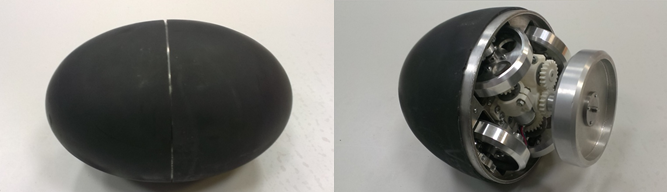
\includegraphics[width=0.9\linewidth]{Photo_BPR.png}%
	\caption{Фотографии безвинтового подводного робота}
	\label{Photo_BPR}
\end{figure}

Управление осуществляется с персонального компьютера (ПК), для которого было разработано специальное программное обеспечение. Для управления роботом необходимо задать направления и скорости вращения каждого из роторов, а также время разгона до заданной скорости. Отдельно осуществляется управление модулями плавучести, которые отвечают за погружение робота.

\section{Описание конструкции водоплавающиего недеформируемого рыбоподобного робота}\label{sec:ch3/sec2}

Робот представляет собой полый объект, в продольном сечении имеющий форму профиля крыла NACA 0040 (см. рисунок \ref{Photo_NACA}) длиной 340 мм, шириной 134 мм. Высота робота 80 мм. Корпус изготовлен на 3Д-принтере из PLA-пластика, толщина стенки -- 2 мм. Внутри корпуса закреплен ротор с двигателем таким образом, что центр масс всей системы находится максимально близко к нижней грани робота. В качестве двигателя использовался мотор-редуктор фирмы Pololu с энкодером. Для передачи вращения с двигателя к ротору использовалась пара шестерен с передаточным отношением 3.5:1. Внутри так же располагается элемент питанияи плата с микроконтроллером модели STM32F303K8, управляющим вращением двигателем постоянного тока. Для управления двигателем используется драйвер двигателя постоянного тока VNH3SP30 фирмы STMicroelectronics. Энкодер использовался для определения положения ротора в течение экспериментов. Дифференцируя данные, полученные с энкодера, можно получить угловую скорость вращения ротора.
%Характеристики двигателя: номинальное напряжение питания -- 6 В, передаточное отношение редуктора -- 47:1, момент на валу -- 0.459 Нм, максимальная скорость вращения -- 120 об/мин. 


\begin{figure}[h]
	\centering
	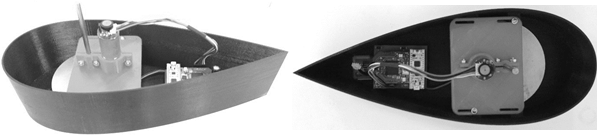
\includegraphics[width=1\linewidth]{Photo_NACA.png}%
	\caption{Безвинтовой рыбоподобный робот}
	\label{Photo_NACA}
\end{figure}

Реальная модель робота имеет следующие характеристики: m = $0.905$ кг; $I_0$ = $0.00844$ кг$\cdot$м2; Ротор изготовлен из алюминия, имеет внешний диаметр 110 мм, высоту 12 мм. Масса ротора $m_r$ = $0.327$ кг; момент инерции ротора $I_r$ = $0.00058$ кг$\cdot$м2. Конструкция робота позволяет смещать центр вращения ротора.

Управление осуществляется с персонального компьютера, для которого было разработано специальное программное обеспечение. Все команды роботу передаются по беспроводному каналу связи, используя Bluetooth.

\clearpage